\documentclass[11pt]{article}
% The report's page layout. The fonts, colours and diagram styles are in figure-style.tex.

% Fonts, colours, TikZ styles and macros that every diagram and plot uses.
% Loaded by style.tex (the report) and by make-diagrams.py (one file per diagram).

\usepackage{amsmath}
\usepackage{newtxmath}
% Tectonic runs XeTeX without system fonts, so load the TeX Gyre fonts by file name:
% Termes (a Times) for the text, Heros (a Helvetica) for headings and labels.
\usepackage{fontspec}
\setmainfont{texgyretermes}[Extension=.otf, UprightFont=*-regular, BoldFont=*-bold,
  ItalicFont=*-italic, BoldItalicFont=*-bolditalic]
\setsansfont{texgyreheros}[Extension=.otf, UprightFont=*-regular, BoldFont=*-bold,
  ItalicFont=*-italic, BoldItalicFont=*-bolditalic, Scale=0.92]

\usepackage{xcolor}
\usepackage{tikz}
\usepackage{pgfplots}
\pgfplotsset{compat=1.18}
\usetikzlibrary{arrows.meta, positioning, fit, calc, shapes.geometric, backgrounds,
  decorations.pathreplacing}

% One palette for every figure: a layer has one colour everywhere.
\definecolor{mcu}{HTML}{E8F1FB}       % motion: the Arduino, drivers, motors, servos
\definecolor{mcuedge}{HTML}{2F6DB5}
\definecolor{host}{HTML}{EAF6EC}      % the computers: the Raspberry Pi and the laptop
\definecolor{hostedge}{HTML}{2E7D32}
\definecolor{ui}{HTML}{FFF4E0}        % interfaces: the phone app, Bluetooth
\definecolor{uiedge}{HTML}{C77700}
\definecolor{vis}{HTML}{F3ECFA}       % vision: camera, dataset, YOLOv8
\definecolor{visedge}{HTML}{7B3FA8}
\definecolor{hw}{HTML}{F1F1F1}        % body and other hardware
\definecolor{hwedge}{HTML}{555555}
\definecolor{warn}{HTML}{FDECEC}
\definecolor{warnedge}{HTML}{B3261E}

\tikzset{
  >={Stealth[length=2mm]},
  box/.style={draw, rounded corners=2pt, align=center, font=\footnotesize,
              minimum height=7mm, inner sep=3pt},
  mcubox/.style={box, fill=mcu, draw=mcuedge},
  hostbox/.style={box, fill=host, draw=hostedge},
  uibox/.style={box, fill=ui, draw=uiedge},
  hwbox/.style={box, fill=hw, draw=hwedge},
  visbox/.style={box, fill=vis, draw=visedge},
  warnbox/.style={box, fill=warn, draw=warnedge},
  group/.style={draw, dashed, rounded corners=3pt, inner sep=6pt},
  grouplabel/.style={font=\scriptsize\itshape, anchor=north west},
  flow/.style={->, thick},
  dataflow/.style={->, thick, densely dashed},
  lbl/.style={font=\scriptsize, midway, fill=white, inner sep=1pt},
}

% A file, function or code name, typeset as written (underscores included).
\newcommand{\topic}[1]{\texttt{\detokenize{#1}}}


% --- Page and type: one column, 11 pt, room to breathe -----------------------
\usepackage[a4paper, margin=25mm, headheight=14pt]{geometry}
\usepackage[final]{microtype}
\usepackage{setspace}
\setstretch{1.15}
\setlength{\parindent}{0pt}
\setlength{\parskip}{0.7\baselineskip}
\setlength{\emergencystretch}{2em}   % room for long code names without overfull lines
\usepackage{enumitem}
\setlist{itemsep=2pt, topsep=4pt}

% --- Colour accents ------------------------------------------------------------
\definecolor{accent}{HTML}{1F5FA8}     % headings, links, the title band
\definecolor{accentsoft}{HTML}{EAF2FB}
\definecolor{ink}{HTML}{22262B}
\definecolor{muted}{HTML}{5F6670}
\color{ink}

\usepackage[font={small,sf}, labelfont={bf,color=accent}, margin=8mm, skip=6pt,
  justification=raggedright, singlelinecheck=true]{caption}
% Let figures share pages with text instead of sitting alone on float pages
\renewcommand{\topfraction}{0.9}
\renewcommand{\bottomfraction}{0.8}
\renewcommand{\textfraction}{0.07}
\renewcommand{\floatpagefraction}{0.85}
\setcounter{topnumber}{3}
\setcounter{totalnumber}{4}
\usepackage[section]{placeins}   % keep each section's floats in that section
\usepackage{needspace}           % \Needspace{n\baselineskip} keeps a heading off the page foot
\usepackage{titlesec}
\usepackage[most]{tcolorbox}

\usepackage{fancyhdr}
\pagestyle{fancy}
\fancyhf{}
\fancyhead[L]{\small\sffamily\color{muted} EnviroBot: design, waste detection and prototype}
\fancyhead[R]{\small\sffamily\color{muted} Technical report, v1.0, October 2026}
\fancyfoot[C]{\small\sffamily\color{muted}\thepage}
\renewcommand{\headrulewidth}{0.4pt}
\renewcommand{\headrule}{{\color{accent!40}\hrule height\headrulewidth}}

% Section headings: sans, accent colour, a thin rule under each section
\titleformat{\section}{\Large\sffamily\bfseries\color{accent}}{\thesection}{0.6em}{}[{\color{accent!30}\titlerule[0.6pt]}]
\titleformat{\subsection}{\large\sffamily\bfseries\color{accent!85!black}}{\thesubsection}{0.6em}{}
\titleformat{\paragraph}[runin]{\sffamily\bfseries\color{ink}}{}{}{}[.]
\titlespacing*{\section}{0pt}{1.6\baselineskip}{0.6\baselineskip}
\titlespacing*{\subsection}{0pt}{1.1\baselineskip}{0.3\baselineskip}
\titlespacing*{\paragraph}{0pt}{0.6\baselineskip}{0.6em}

% Status labels, one colour each, used in the results box and the tables
\newcommand{\chip}[2]{\tikz[baseline=(c.base)]\node[fill=#1!15, draw=#1!70!black, text=#1!60!black,
  rounded corners=2pt, inner xsep=3pt, inner ysep=1.2pt, font=\scriptsize\sffamily\bfseries] (c) {#2};}
\newcommand{\measured}{\chip{green!60!black}{measured}}
\newcommand{\onvideo}{\chip{blue}{shown on video}}
\newcommand{\built}{\chip{gray}{built}}

% A soft, coloured box for summaries
\newtcolorbox{summarybox}[1]{colback=accentsoft, colframe=accent, boxrule=0.6pt, arc=2pt,
  left=8pt, right=8pt, top=6pt, bottom=6pt, fonttitle=\sffamily\bfseries, title={#1},
  before upper={\setlength{\parskip}{5pt}}}

% --- Content --------------------------------------------------------------------
\usepackage{graphicx}
\usepackage{adjustbox}
\usepackage{booktabs}
\usepackage{array}
\usepackage{tabularx}
\usepackage{colortbl}
\usepackage{url}
\usepackage{cite}
\usepackage[colorlinks, linkcolor=accent, citecolor=accent, urlcolor=accent]{hyperref}

\graphicspath{{../media/}}

% Table headers in a light accent band
\newcommand{\thead}[1]{\cellcolor{accentsoft}\sffamily\bfseries\small #1}

% A diagram at its natural size, shrunk only if it is wider than the text.
\newcommand{\diagram}[1]{\adjustbox{max width=\textwidth}{\input{#1}}}
% A diagram scaled, up or down, to a share of the text width: \diagramw{0.8}{figures/x}
\newcommand{\diagramw}[2]{\adjustbox{width=#1\textwidth}{\input{#2}}}


\begin{document}

% ---------------------------------------------------------------------------
% Title block
\thispagestyle{empty}
\begin{tcolorbox}[colback=accent, colframe=accent, arc=3pt, left=14pt, right=14pt, top=14pt, bottom=12pt]
  \color{white}\sffamily\raggedright
  {\small Technical report \quad$\cdot$\quad Version 1.0 \quad$\cdot$\quad October 2026}\par\vspace{8pt}
  {\LARGE\bfseries EnviroBot: A Mobile Robotic Arm that Detects and Picks Up Waste}\par\vspace{6pt}
  {\large Design, YOLOv8 Waste Detection and Prototype}
\end{tcolorbox}

\vspace{4pt}
{\sffamily\raggedright
\textbf{Jewel Nath}$^{1,2}$, \textbf{Tasmiara Jahan Toma}$^{2}$, \mbox{\textbf{Tanjina Akter}$^{2}$}\\[2pt]
{\small\color{muted}$^{1}$Independent researcher, Dhaka, Bangladesh\quad $^{2}$Department of Information and Communication Technology, Comilla University, Cumilla, Bangladesh}\\
{\small\color{muted}Jewel Nath: ORCID \href{https://orcid.org/0009-0002-6609-6378}{0009-0002-6609-6378}\quad$\cdot$\quad Code: \url{https://github.com/jewel-nath/envirobot}}\\
{\small\color{muted}Licence: \href{https://creativecommons.org/licenses/by/4.0/}{CC BY 4.0}}\par}

\vspace{6pt}
\begin{summarybox}{Abstract}
EnviroBot is a mobile robot built to find waste on the floor and pick it up. It was built in 2023--24 at Comilla University, Bangladesh, by a team of three students: a four-wheel rover on a stainless steel base carries a six-servo aluminium arm with a gripper, a bin, and a camera.

The robot splits its work between two controllers. In its design, a Raspberry~Pi~3~B handles vision; an Arduino Uno drives the arm through a PCA9685 servo driver and the wheels through two BTS7960 motor drivers, and takes commands over a serial link from the Pi and over Bluetooth from a phone app. Waste is found by a YOLOv8 model trained on 1,700 labelled images in three classes, plastic, paper and trash. The arm is modelled in URDF for ROS~2, and the design plans its motion with MoveIt.

In the team's evaluation, the model labelled 91\% of paper, 94\% of plastic and 92\% of trash objects correctly; when it reported an object where there was none, it most often called it trash. On video, the detector, run on a laptop, labels waste in a live camera view, and the robot's arm picks objects up off the floor. This report describes the robot's mechanical build, electronics, control, arm model and waste detection, presents the evaluation, and sets out the lessons and the next steps toward collecting waste on its own.

\smallskip
{\sffamily\small\textbf{Keywords:} mobile manipulation, waste detection, YOLOv8, robotic arm, ROS~2, MoveIt, Arduino, Raspberry Pi, service robots.}
\end{summarybox}

% ---------------------------------------------------------------------------
\section{Introduction}

Litter on the floors of schools, offices and public places is still picked up by hand. Robots that find litter with a camera and pick it up have been shown in research~\cite{bai2018garbage}, and modern object detectors such as YOLO~\cite{redmon2016yolo} make the finding part fast enough to run in real time. Building such a robot, however, means joining several pieces that are usually studied apart: a mobile base, an arm, a detector, and the control that ties them together.

EnviroBot is a student team's answer to that problem at a low cost. Its aim was a robot that finds waste, labels what kind it is, and picks it up with an arm into a bin it carries (Fig.~\ref{fig:hero}). The team chose off-the-shelf parts available in Bangladesh: an aluminium arm kit, hobby gear motors, a Raspberry~Pi and an Arduino.

\begin{figure}[htbp]
  \centering
  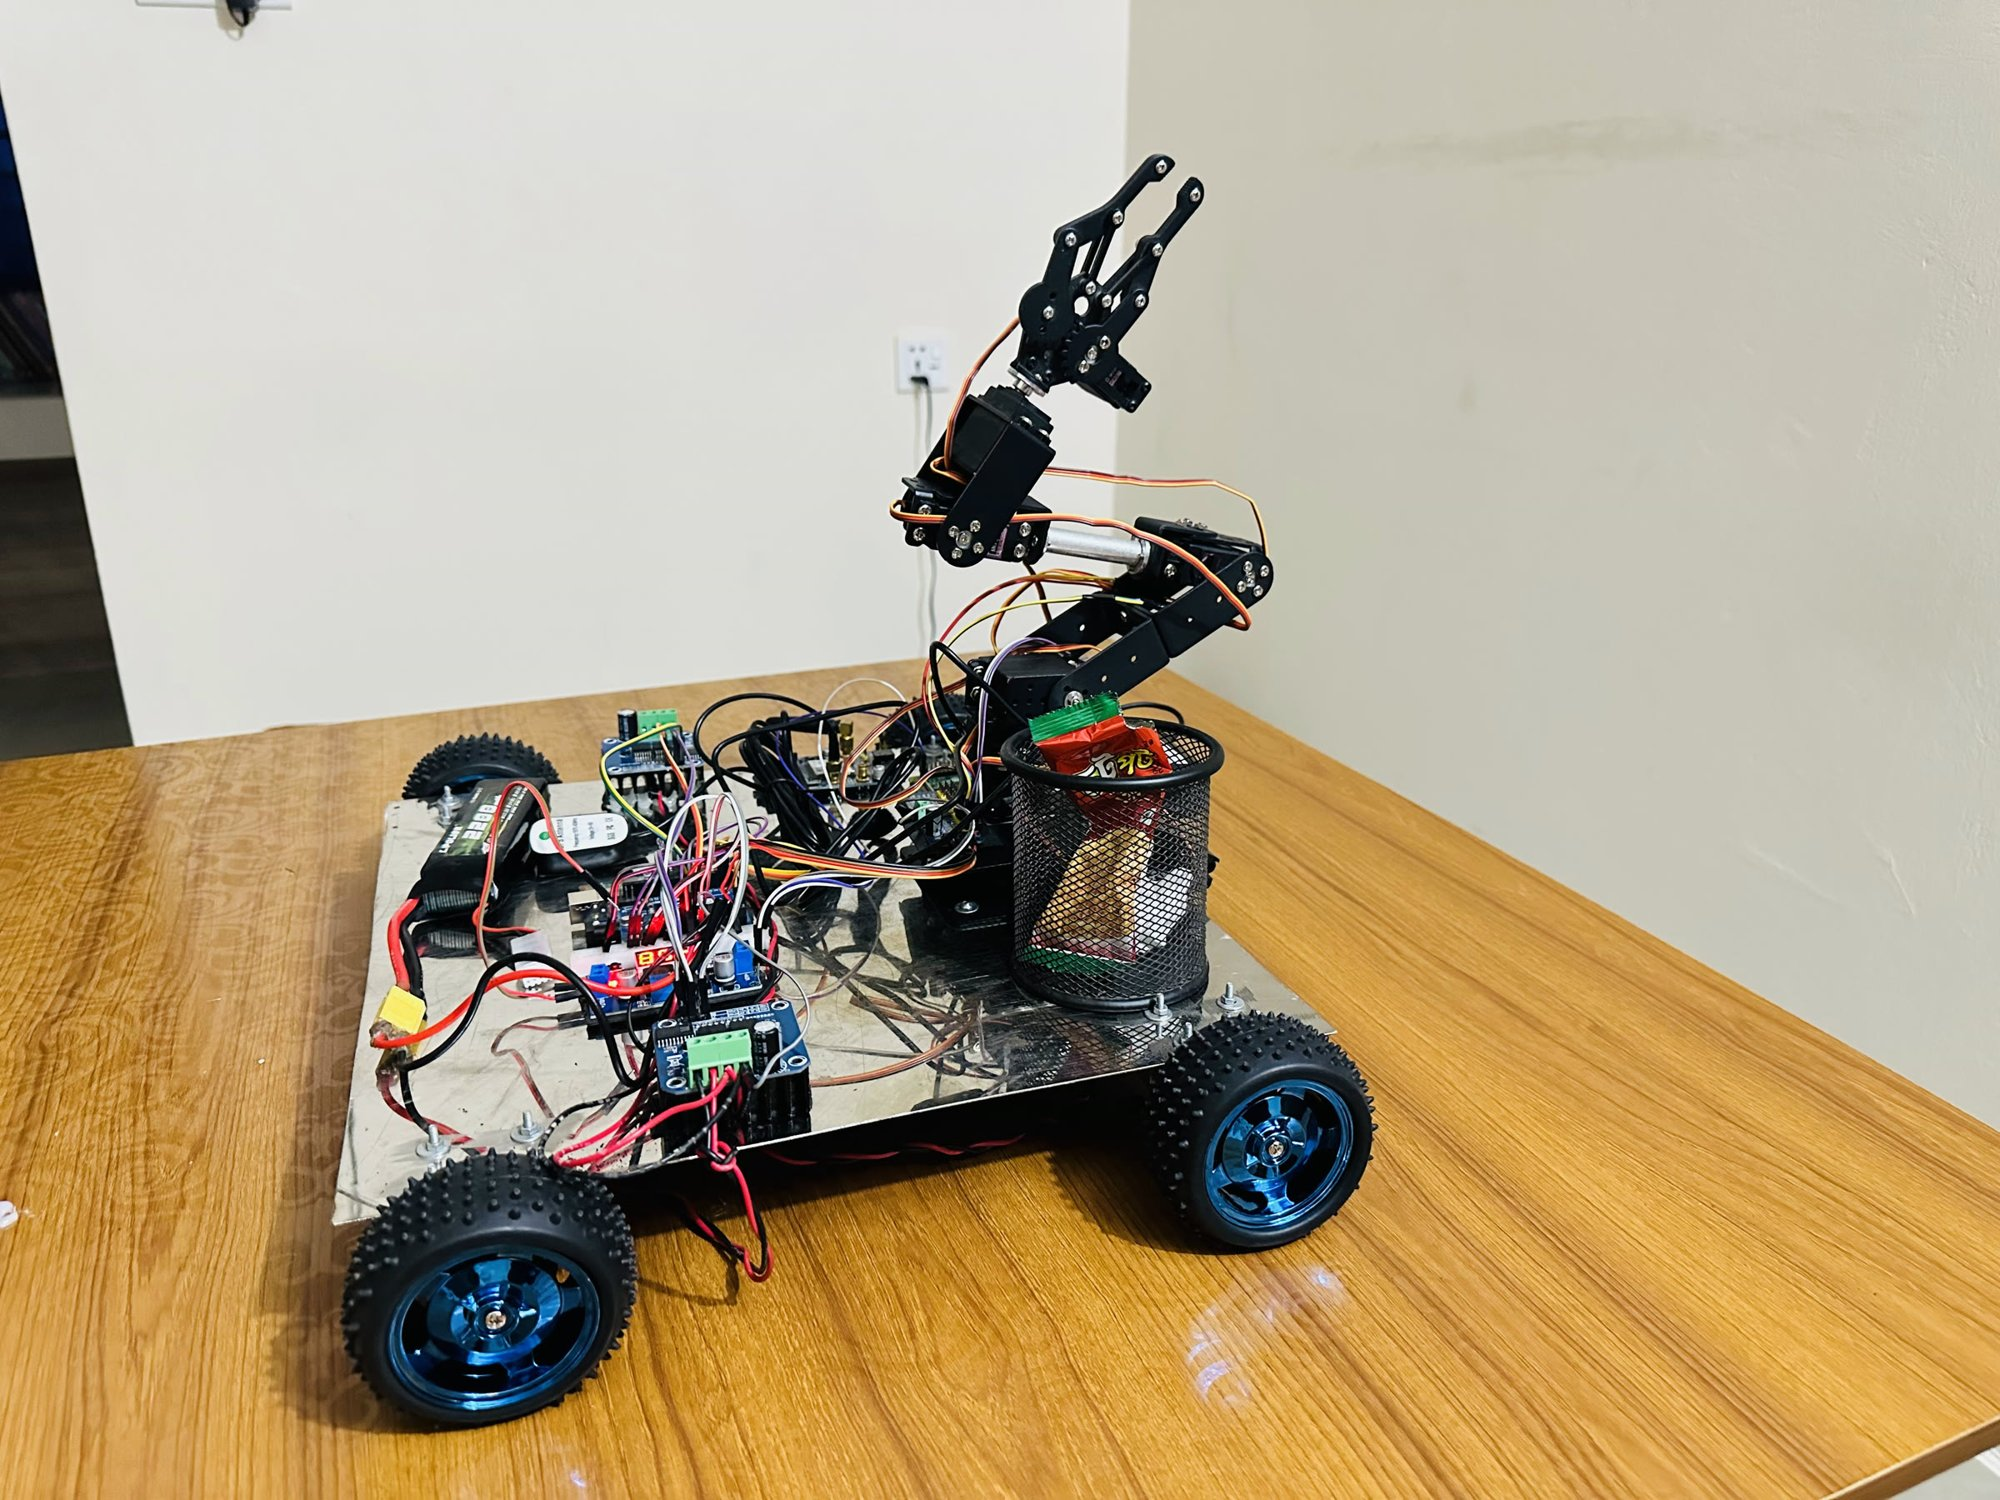
\includegraphics[height=62mm]{envirobot-2024-01-11-finished-robot-side.jpg}\hspace{4mm}
  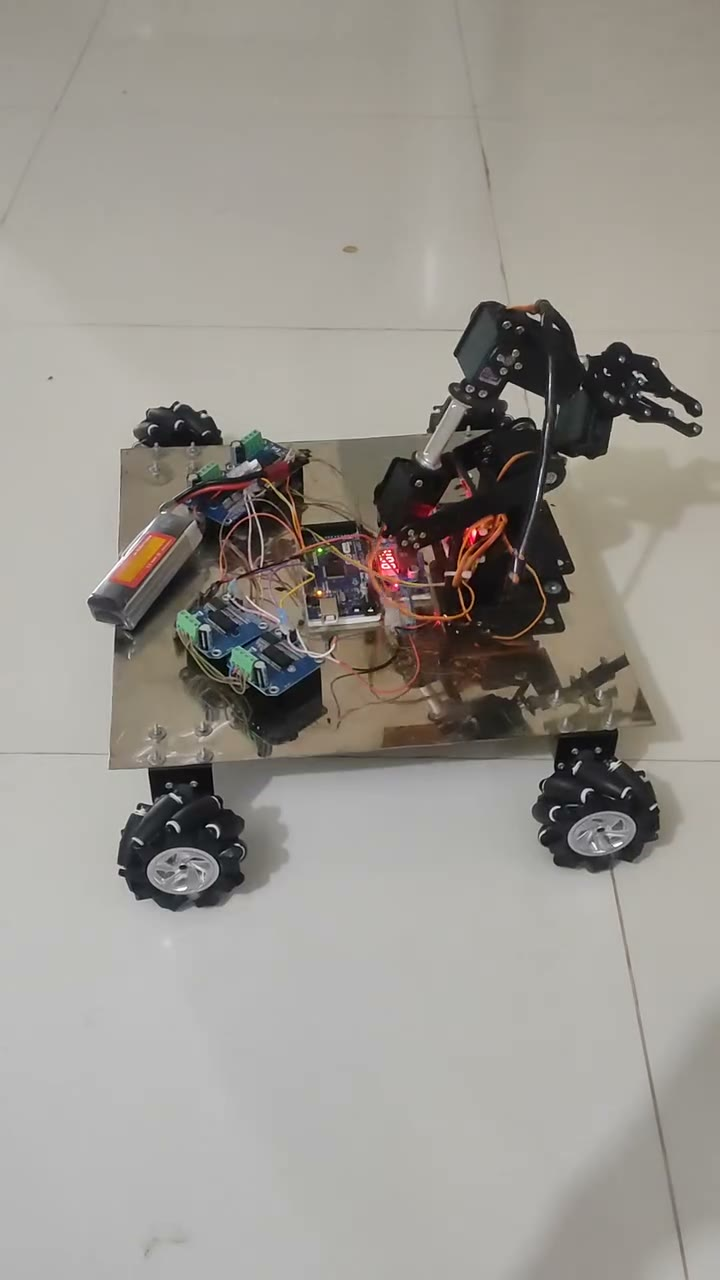
\includegraphics[height=62mm, trim=0 120 0 220, clip]{envirobot-2024-05-11-driving-test-frame.jpg}
  \caption{EnviroBot, finished, on 11 January 2024: the arm raised over the mesh bin, the electronics on the steel base (left). In a later driving test, on 11 May 2024, the arm rides on a base with mecanum wheels (right).}
  \label{fig:hero}
\end{figure}

This report describes EnviroBot as built, and contributes:

\begin{enumerate}
  \item a mobile manipulator built from low-cost parts: a 14-inch steel rover with four gear motors carrying a six-servo arm and a bin (Section~\ref{sec:build});
  \item a two-controller design that keeps vision on a Raspberry~Pi and all motion on an Arduino, joined by a serial link, with manual control from a phone app over Bluetooth (Sections~\ref{sec:electronics}--\ref{sec:control});
  \item the arm modelled in URDF for ROS~2, moved joint by joint in RViz, with motion planning by MoveIt in the design (Section~\ref{sec:model});
  \item a YOLOv8 waste detector trained on 1,700 images in three classes, and its evaluation (Sections~\ref{sec:detection}--\ref{sec:eval});
  \item the behaviours shown on video, and the open source model of the robot, under the MIT licence~\cite{envirobotrepo} (Section~\ref{sec:demo}).
\end{enumerate}

\begin{summarybox}{Results at a glance}
\renewcommand{\arraystretch}{1.25}
\small
\begin{tabularx}{\linewidth}{@{}>{\raggedright\arraybackslash}p{0.3\linewidth}X>{\raggedleft\arraybackslash}p{0.2\linewidth}@{}}
  \textbf{\sffamily What EnviroBot does} & \textbf{\sffamily How} & \textbf{\sffamily Evidence} \\
  \midrule
  Labels waste by type & YOLOv8: 91\% of paper, 94\% of plastic and 92\% of trash objects labelled correctly & \measured \\
  Finds waste in a live camera view & the detector boxes and names objects as they come into view & \onvideo \\
  Picks objects off the floor & the six-servo arm reaches down, grips and lifts & \onvideo \\
  Drives and moves its arm from a phone & an MIT App Inventor app over Bluetooth & \built \\
  Models the arm for ROS~2 & the arm's URDF model, moved joint by joint in RViz & \built \\
  Drives on mecanum wheels & a later driving test of the rover with its arm & \onvideo \\
\end{tabularx}
\par\smallskip
{\footnotesize\sffamily The evaluation is the team's own, from their report of 14 January 2024. The videos were recorded on 11 January and 11 May 2024.}
\end{summarybox}

% ---------------------------------------------------------------------------
\section{Related Work}

\paragraph{Robots that collect litter} Bai et al.\ built a robot that finds garbage on grass with a deep network and picks it up with an arm~\cite{bai2018garbage}. EnviroBot follows the same pattern, a detector on board a mobile base that guides an arm, on indoor floors and with low-cost parts.

\paragraph{Detecting waste} YOLO frames detection as one pass of a network over the image~\cite{redmon2016yolo}; YOLOv8~\cite{yolov8} is the version EnviroBot uses. General detectors are trained on datasets such as COCO~\cite{lin2014coco}; for waste, TrashNet~\cite{yang2016trashnet} classifies photos of single items into six classes, and TACO~\cite{proenca2020taco} annotates litter in the wild. EnviroBot's dataset, like TrashNet, has a few material classes.

\paragraph{Arms on ROS} ROS~2~\cite{macenski2022ros2} is the common middleware for robots today, and MoveIt~\cite{coleman2014moveit} its motion-planning framework. Megalingam et al.\ modelled and controlled a 6-DOF arm in ROS~\cite{megalingam2018arm}, the approach EnviroBot takes for its arm.

% ---------------------------------------------------------------------------
\section{System Overview}
\label{sec:overview}

Fig.~\ref{fig:overview} shows the whole robot. Two controllers share the work. In the design, the Raspberry~Pi is the vision computer: it reads the camera and runs the detector (in the recorded test, the detector ran on a laptop). The Arduino Uno is the motion controller: it sets the six arm servos through a PCA9685 servo driver~\cite{pca9685} over I$^2$C, and the four wheel motors through two BTS7960 motor drivers~\cite{bts7960}. The Pi and the Arduino talk over a serial link; a phone app sends the Arduino commands over Bluetooth. A 3-cell LiPo battery powers the robot.

\begin{figure}[htbp]
  \centering
  \diagramw{0.98}{figures/fig01-system-overview}
  \caption{System overview. The Raspberry~Pi (green) handles vision (purple); the Arduino drives the arm and the wheels (blue); the phone app (orange) gives manual control. From the team's circuit diagram and parts list.}
  \label{fig:overview}
\end{figure}

The split follows from what each board does well. The Pi runs Linux, Python and the detector; the Arduino gives steady, timed output to the drivers, and lets the phone drive the robot without the Pi.

% ---------------------------------------------------------------------------
\section{Mechanical Build}
\label{sec:build}

\paragraph{The rover} The arm is heavy for a small robot, so the team built a sturdy base: a 14 by 14 inch (356\,mm) stainless steel sheet with a 12\,V gear motor at each corner, each rated at 300\,rpm with a torque sold as ``10\,kg'' (Figs.~\ref{fig:build} and~\ref{fig:layout}). Each of the two motor drivers runs a pair of the motors.

\paragraph{The arm} The arm is an aluminium six-servo kit with a clamp claw: a waist, a shoulder, an elbow, a wrist that pitches and rolls, and a gripper. It is fixed at the front of the base, so that it reaches the floor in front of the robot without the base in its way. A mesh bin sits on the base beside it, within the arm's reach.

\begin{figure}[htbp]
  \centering
  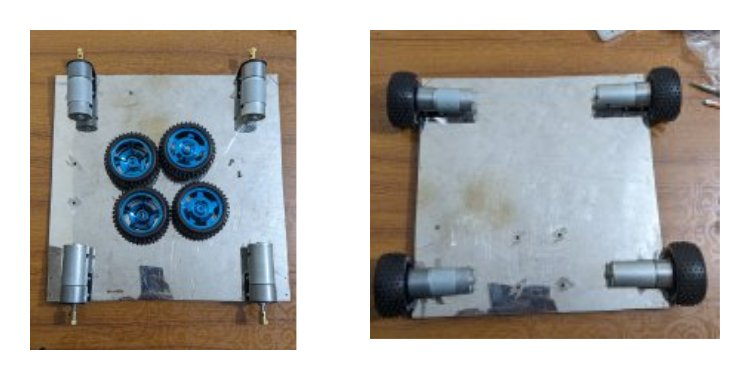
\includegraphics[height=29mm]{envirobot-2024-01-14-report-rover-base.jpg}\hfill
  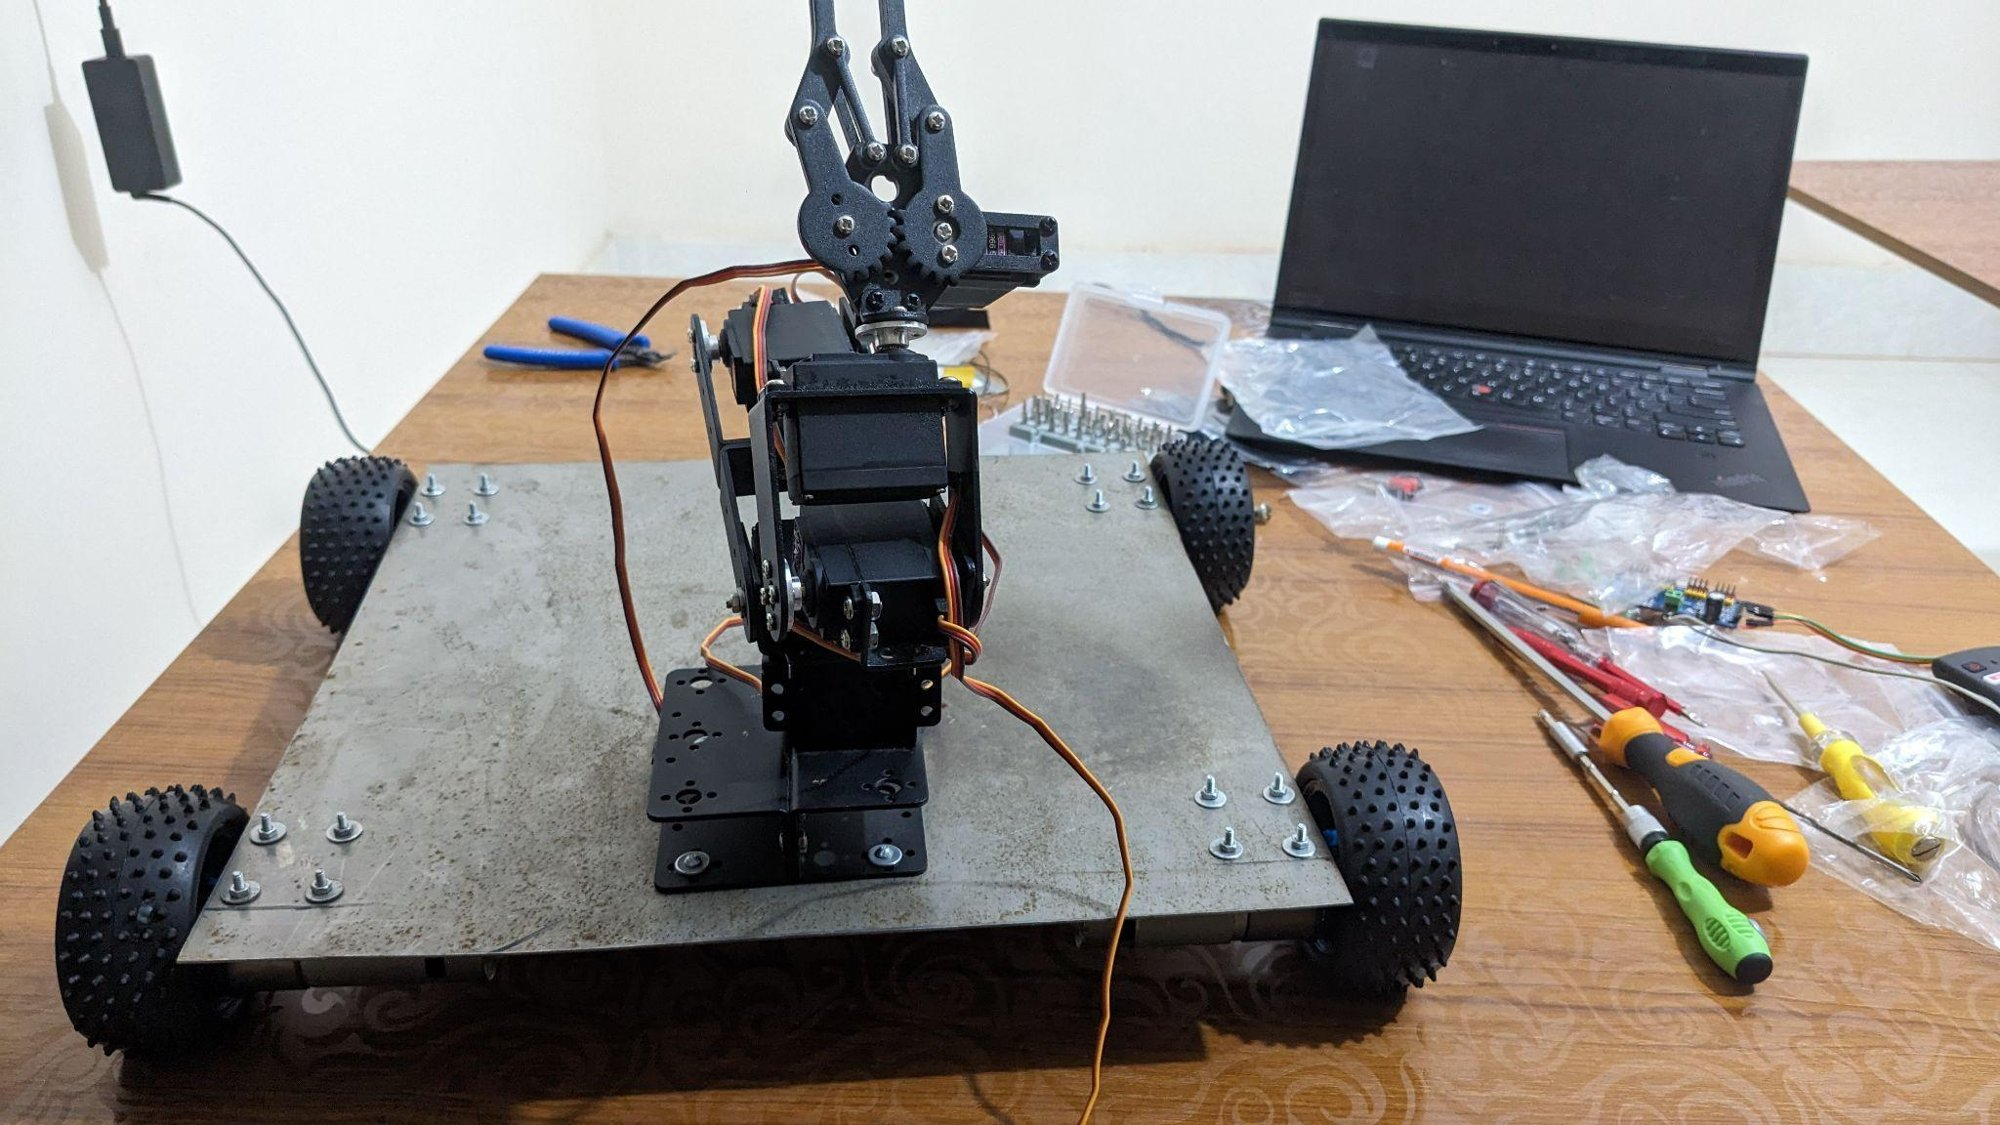
\includegraphics[height=29mm]{envirobot-2024-01-14-report-arm-on-rover-build.jpg}\hfill
  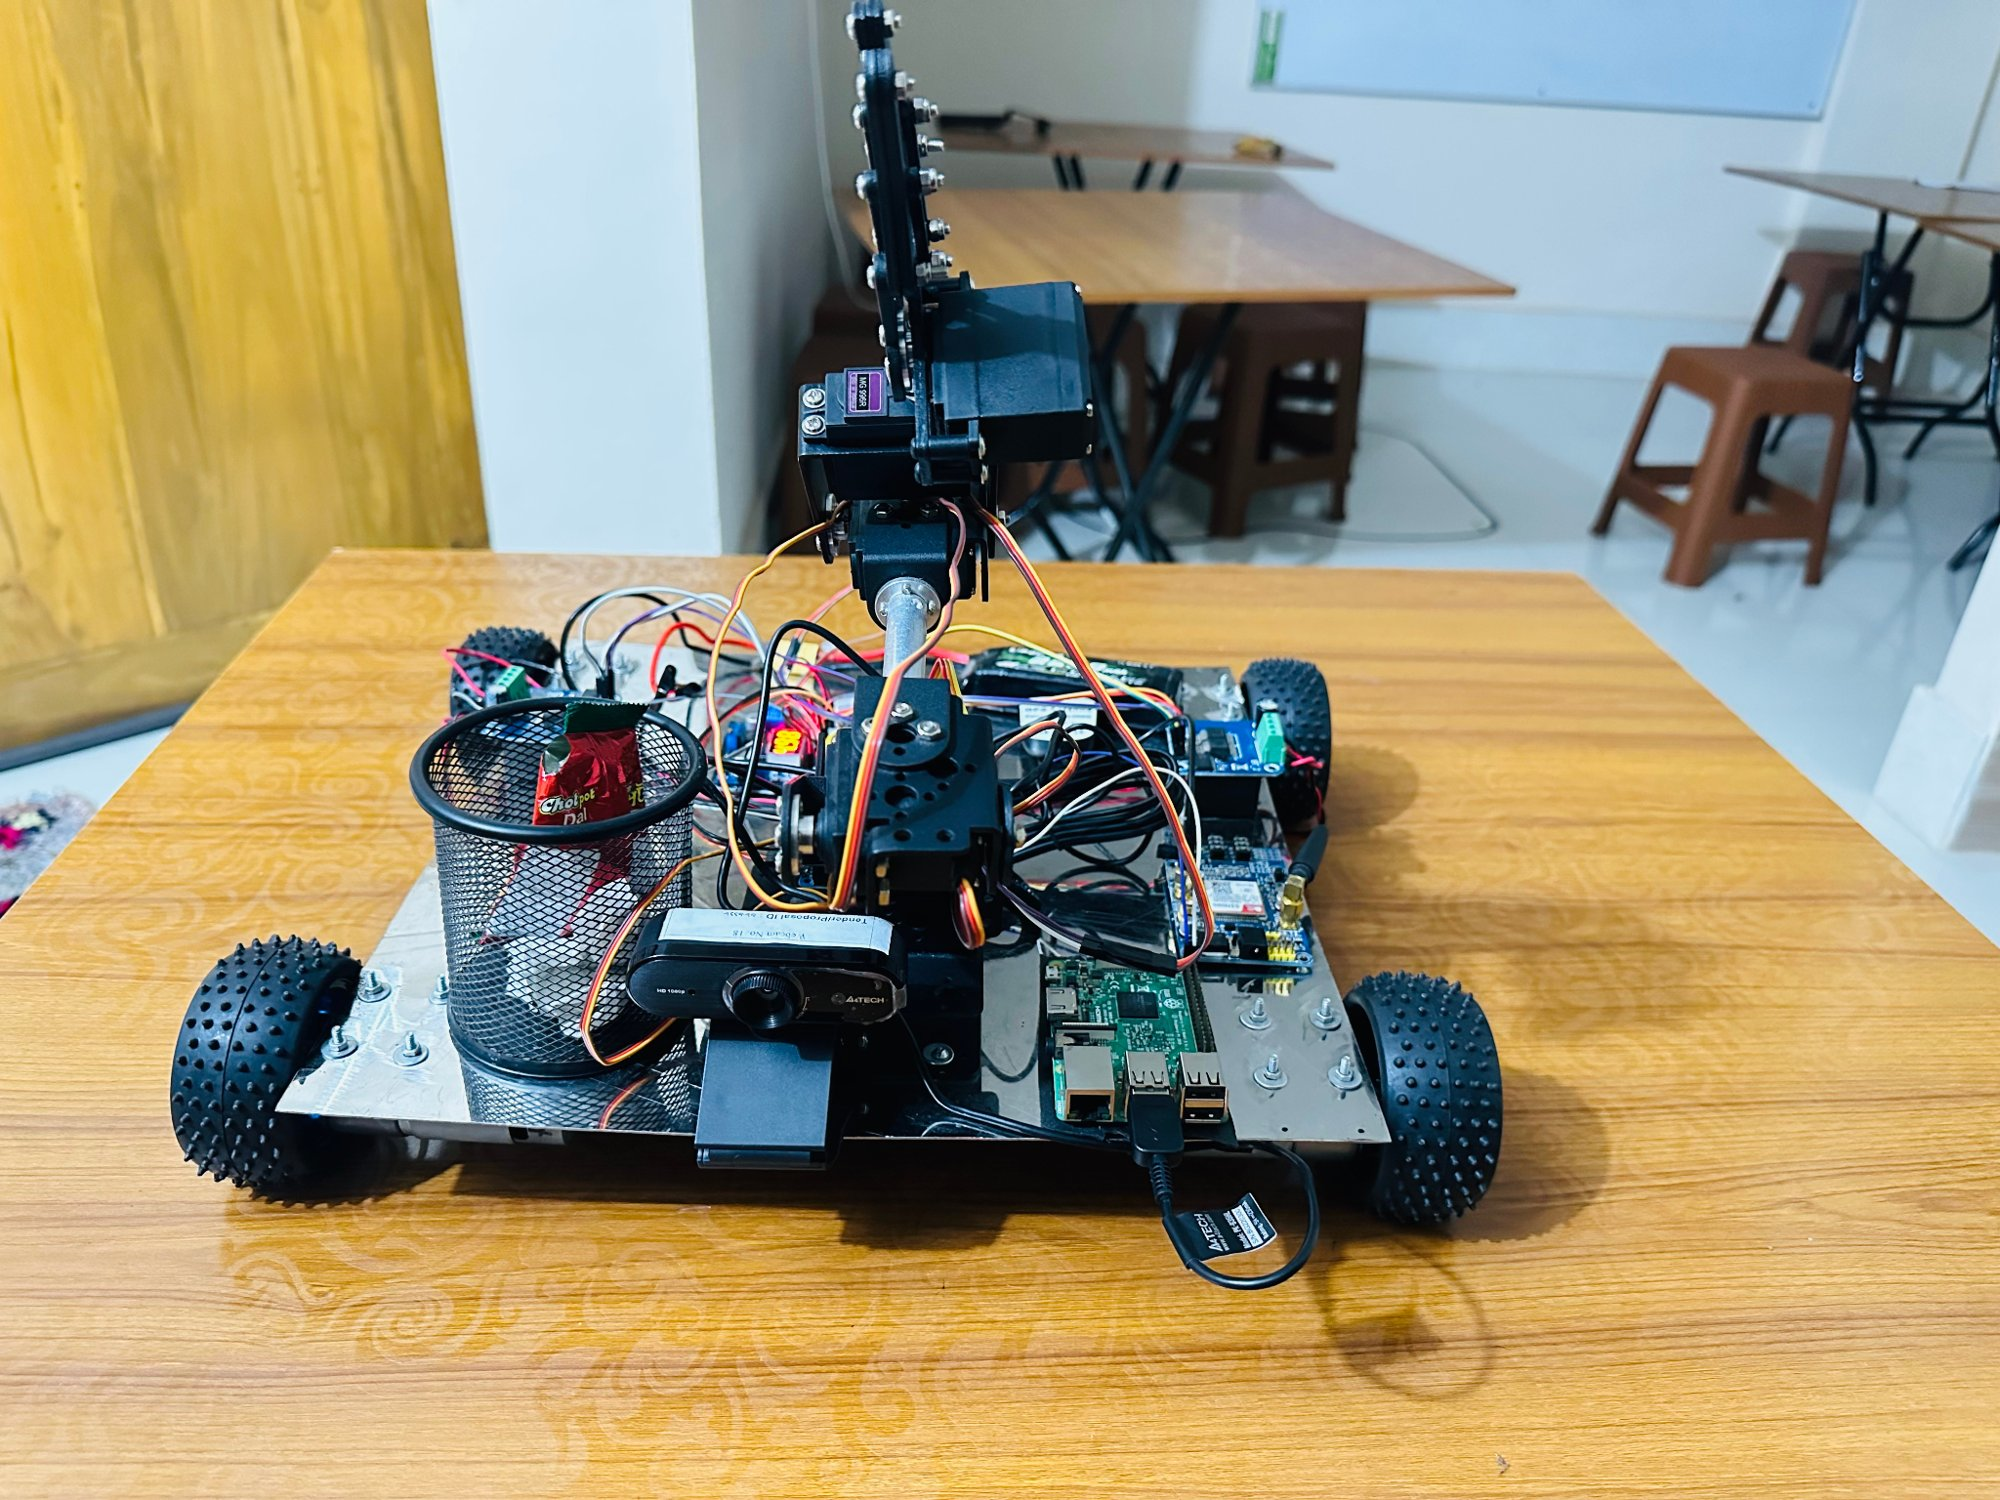
\includegraphics[height=29mm]{envirobot-2024-01-14-report-finished-robot-1.jpg}
  \caption{The build: the steel base with its four gear motors and wheels, from below and above (left); the arm fitted at the front of the base (middle); the finished robot with its bin, camera and boards (right).}
  \label{fig:build}
\end{figure}

\begin{figure}[htbp]
  \centering
  \diagramw{0.4}{figures/fig04-rover-layout}
  \caption{The rover from above, to scale for the base. The arm sits at the front; the positions of the bin, the electronics and the battery are drawn schematically.}
  \label{fig:layout}
\end{figure}

Fig.~\ref{fig:timeline} places the build in time, from the earliest dated image of the arm's model, in September 2023, to the finished robot in January 2024 and a later driving test on mecanum wheels in May 2024.

\begin{figure}[htbp]
  \centering
  \diagramw{0.98}{figures/fig09-timeline}
  \caption{EnviroBot from the earliest dated image of the arm's model to the later driving test, from the dated photos, videos, report and repository.}
  \label{fig:timeline}
\end{figure}

% ---------------------------------------------------------------------------
\section{Electronics}
\label{sec:electronics}

Table~\ref{tab:hw} lists the main parts, and Fig.~\ref{fig:wiring} the wiring, from the team's circuit diagram of 14 January 2024. The Pi's UART (pins 8 and 10) is crossed to the Arduino's serial pins; the camera plugs into the Pi's USB port. The Arduino reaches the PCA9685 on its I$^2$C pins, A4 and A5, and sends PWM to the two BTS7960 drivers on pins 11 and 10 for the first and 6 and 5 for the second; each driver runs two motors. The drivers' enable pins are tied high, and their motor supply is the 12\,V line from the 3-cell battery.

\begin{figure}[htbp]
  \centering
  \diagramw{0.98}{figures/fig02-wiring}
  \caption{The wiring, pin by pin, from the team's circuit diagram (14 January 2024). The Bluetooth module is described in the report but not drawn in the diagram.}
  \label{fig:wiring}
\end{figure}

\begin{table}[htbp]
  \centering
  \caption{Main parts, from the team report, the circuit diagram and the build photos.}
  \label{tab:hw}
  \renewcommand{\arraystretch}{1.25}
  \small
  \begin{tabularx}{0.92\textwidth}{@{}>{\sffamily\bfseries}p{0.24\textwidth}X@{}}
    \toprule
    \thead{Part} & \thead{Role} \\
    \midrule
    Raspberry Pi 3 B & vision computer in the design: the camera and the detector \\
    Arduino Uno & motion controller: the arm and the wheels; serial to the Pi, Bluetooth to the phone \\
    PCA9685 & 16-channel, 12-bit PWM servo driver on I$^2$C; six channels used \\
    6 servos & the arm kit's joints: waist, shoulder, elbow, wrist pitch, wrist roll, gripper \\
    2 $\times$ BTS7960 & H-bridge motor drivers, one per pair of wheels \\
    4 gear motors & 12\,V, 300\,rpm, torque sold as ``10\,kg'', one per wheel \\
    Camera & a USB webcam under the arm (the report also lists a Kinect sensor) \\
    LiPo battery & 3 cells, 11.1\,V, 2200\,mAh \\
    Bluetooth module & on the Arduino, for the phone app \\
    \bottomrule
  \end{tabularx}
\end{table}


% ---------------------------------------------------------------------------
\section{Control from a Phone}
\label{sec:control}

Before any autonomy, the team made the robot fully controllable by hand, which let them test every joint and the drive on their own. The app, built in MIT App Inventor~\cite{appinventor}, connects to the Arduino over Bluetooth (Fig.~\ref{fig:app}). Its arm screen has a pair of buttons for each joint, grip, wrist pitch, wrist roll, elbow, shoulder and waist, a slider for the arm's speed, and buttons to save a sequence of positions, run it back, and reset. Other buttons drive the rover.

\begin{figure}[htbp]
  \centering
  \begin{minipage}[c]{0.3\textwidth}
    \centering
    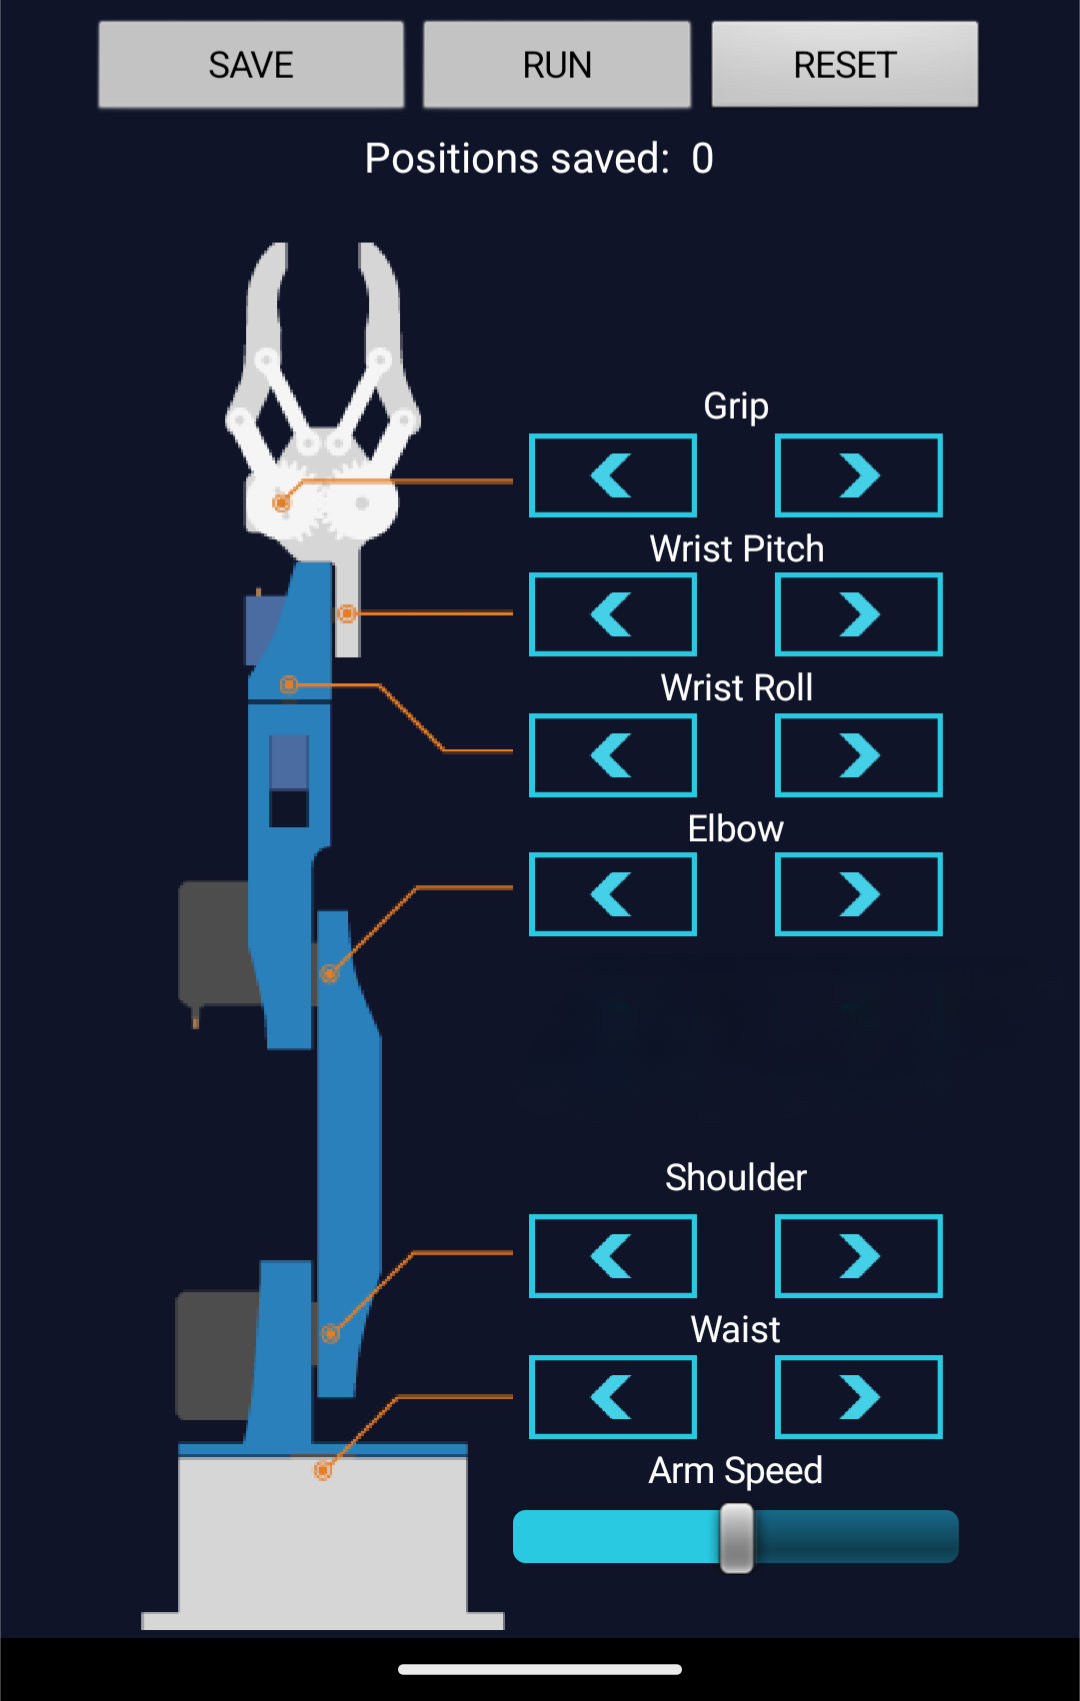
\includegraphics[width=0.85\linewidth]{envirobot-2024-01-14-report-control-app.png}
  \end{minipage}\hfill
  \begin{minipage}[c]{0.66\textwidth}
    \centering
    \diagram{figures/fig05-app-control}
  \end{minipage}
  \caption{Manual control. The app's arm screen (left): a pair of buttons for each joint, a speed slider, and Save, Run and Reset. Each command goes over Bluetooth to the Arduino, which moves a joint through the servo driver or the wheels through the motor drivers (right).}
  \label{fig:app}
\end{figure}

The motors and servos were brought up step by step. Each motor was tested with its driver from the Arduino's serial monitor, and its wiring or code corrected until it turned the right way. Each servo was calibrated the same way: its starting, lowest and highest angles were found and written down, so the arm's commands stay within each joint's range.

% ---------------------------------------------------------------------------
\Needspace{10\baselineskip}
\section{Arm Model and Motion Planning}
\label{sec:model}

The arm is described in URDF, through xacro, as a ROS~2 package, \topic{smart_arm}~\cite{macenski2022ros2,envirobotrepo}. Its chain has six controlled joints, from the waist to the gripper, plus a second finger joint that mirrors the first, so one servo opens and closes both fingers (Fig.~\ref{fig:chain}). Each joint has limits on its travel. A second file models the rover base, with a continuous joint for each wheel.

\begin{figure}[htbp]
  \centering
  \diagramw{0.85}{figures/fig03-arm-chain}
  \caption{The arm's kinematic chain in the URDF model: links (grey) and joints (blue), each joint named as on the app's arm screen, with its axis and its range in degrees.}
  \label{fig:chain}
\end{figure}

The team first moved the model joint by joint in RViz, with a slider for each joint, in September 2023. The team report describes the next step, setting the arm up in MoveIt~\cite{coleman2014moveit}, which plans a collision-free path for the arm to a goal pose (Fig.~\ref{fig:rviz}). A ros2\_control set-up names the same six joints for a joint-trajectory controller; it is not yet wired into the model.

\begin{figure}[htbp]
  \centering
  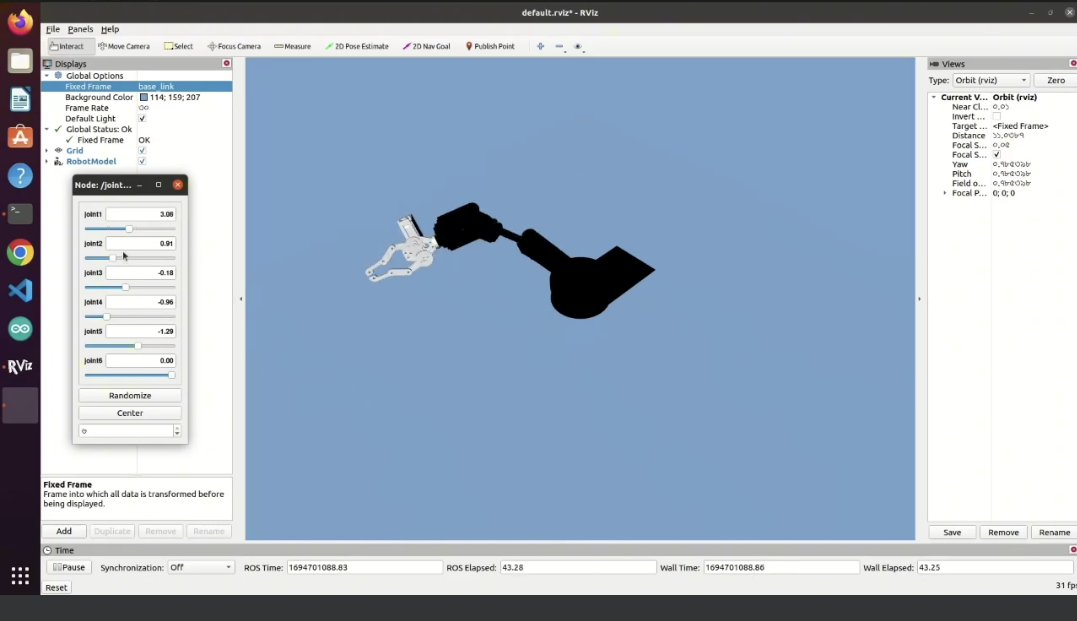
\includegraphics[height=60mm]{envirobot-2023-09-14-arm-model-rviz.jpg}
  \caption{The arm's model in RViz, moved with a slider for each joint, on 14 September 2023.}
  \label{fig:rviz}
\end{figure}

The team designed the full autonomous pick-up on this base (Fig.~\ref{fig:pipeline}): a ROS~2 node runs the detector on each camera frame and passes on the class and position of each item; a target is chosen from it; MoveIt plans the arm's path to it; and the Arduino moves the joints along the plan. Two of these parts were shown on their own: the detector, running live on a laptop, and the arm picking an object up off the floor, as Sections~\ref{sec:eval} and~\ref{sec:demo} describe. Planning with MoveIt stayed in the design; setting it up and joining the parts into one program are the next steps (Section~\ref{sec:future}).

\begin{figure}[htbp]
  \centering
  \diagramw{0.98}{figures/fig06-autonomy-pipeline}
  \caption{The autonomous pick-up, as designed: from a camera frame to the arm, through the detector, a chosen target and MoveIt.}
  \label{fig:pipeline}
\end{figure}

% ---------------------------------------------------------------------------
\section{Waste Detection with YOLOv8}
\label{sec:detection}

\paragraph{Data} The team's dataset holds 1,700 images in three classes, plastic, paper and trash, many of them from an earlier project in their department (Fig.~\ref{fig:dataset}). Each item in each image is labelled with a box and a class. The set was enlarged by changing the brightness of some images and shifting and rotating others, and every image was resized to 512 by 384 pixels with OpenCV. It was split 70/20/10 into training, validation and test sets.\footnote{The report gives the split as 1,226, 350 and 176 images, which add up to 1,752 rather than 1,700; the report does not explain the difference.}

\paragraph{Model} The detector is YOLOv8~\cite{yolov8} in its large size, YOLOv8l, trained for 50 epochs in Google Colab. YOLOv8 finds the objects in an image and classifies them in one pass of the network~\cite{redmon2016yolo}; its loss combines binary cross-entropy for the classes with distribution focal and CIoU losses for the boxes.

\begin{figure}[htbp]
  \centering
  \diagramw{0.8}{figures/fig07-dataset-pipeline}
  \caption{From images to a trained detector: labelling, augmentation, resizing, the split, and training YOLOv8l.}
  \label{fig:dataset}
\end{figure}

% ---------------------------------------------------------------------------
\section{Evaluation}
\label{sec:eval}

The team's report of 14 January 2024 gives the training curves and a confusion matrix; the figures below are typed in from it. The report does not say which split the matrix was computed on.

\paragraph{Training} Accuracy rose unevenly at first, with sharp drops at epochs 5--6, 19 and 30, then settled from epoch 34 and reached 0.81 by epoch 50; the loss fell from 2.57 to 0.37, with a clear step down after epoch 40 (Fig.~\ref{fig:training}). The report does not name the accuracy metric, so this curve is best read as the trend of training rather than a measure to compare with other detectors.

\begin{figure}[htbp]
  \centering
  \diagramw{0.62}{figures/plot01-training-accuracy}\par\medskip
  \diagramw{0.62}{figures/plot02-training-loss}
  \caption{Training over 50 epochs: the accuracy the team reported (top) and the loss (bottom). Values read off the report's charts, to about $\pm$0.02.}
  \label{fig:training}
\end{figure}

\paragraph{Per class} The confusion matrix (Fig.~\ref{fig:cm}) shows, for the objects of each true class, the share given each label. The model labelled 91\% of paper objects, 94\% of plastic and 92\% of trash correctly; confusions between the three classes were at most 5\%, and a few paper and trash objects (3\% and 1\%) were missed as background.

\begin{figure}[htbp]
  \centering
  \diagramw{0.5}{figures/fig08-confusion-matrix}
  \caption{The detector's confusion matrix, from the team report. Each column is one true class and sums to 1, to rounding; the diagonal is the share labelled correctly. The background column shows what the model's false detections were labelled.}
  \label{fig:cm}
\end{figure}

The background column tells the rest of the story. When the model reported an object where there was none, it called it trash half the time (0.50), plastic 30\% and paper 20\%. Trash, the broadest of the three classes, drew the most.

\begin{summarybox}{Key finding}
The detector tells waste types apart well: 91--94\% of the objects in each class were labelled correctly, and no two classes were confused more than 5\% of the time. When it reported an object where there was none, it most often called it trash; more background images in training might reduce this.
\end{summarybox}

% ---------------------------------------------------------------------------
\section{Demonstrations}
\label{sec:demo}

The robot's abilities were recorded on video (Table~\ref{tab:demo}, Fig.~\ref{fig:demo}).

\begin{table}[htbp]
  \centering
  \caption{Behaviours recorded on video.}
  \label{tab:demo}
  \renewcommand{\arraystretch}{1.3}
  \small
  \begin{tabularx}{\textwidth}{@{}>{\sffamily}p{0.13\textwidth}>{\raggedright\arraybackslash}X@{}}
    \toprule
    \thead{Date} & \thead{What the video shows} \\
    \midrule
    11 Jan 2024 & The detector running live on a laptop, boxing and naming objects as they come into view (42\,s) \\
    11 Jan 2024 & The arm reaching down from the rover, gripping a small cube off the floor and lifting it (73\,s) \\
    11 Jan 2024 & An arm test on the floor: the arm reaching down to a small box on the floor (77\,s) \\
    11 Jan 2024 & Close-ups of the finished robot: the arm, the bin, the battery and the boards (20\,s) \\
    11 May 2024 & A driving test of the rover with its arm, on mecanum wheels (16\,s) \\
    \bottomrule
  \end{tabularx}
\end{table}

\begin{figure}[htbp]
  \centering
  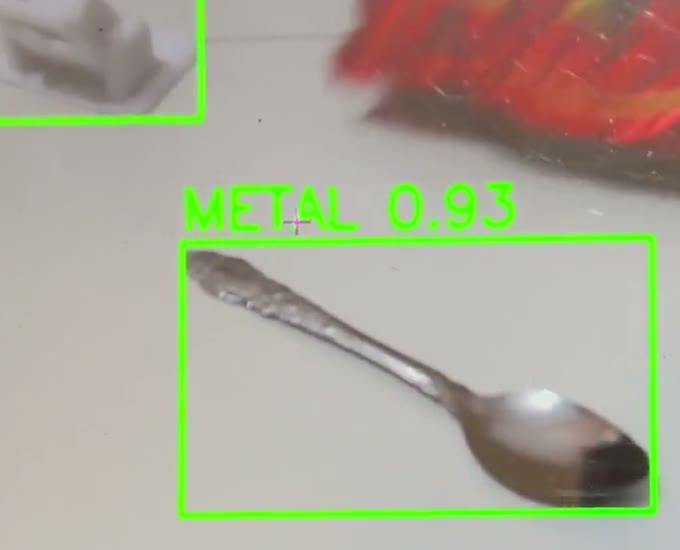
\includegraphics[height=44mm]{envirobot-2024-01-11-yolo-detection-test-poster.jpg}\hfill
  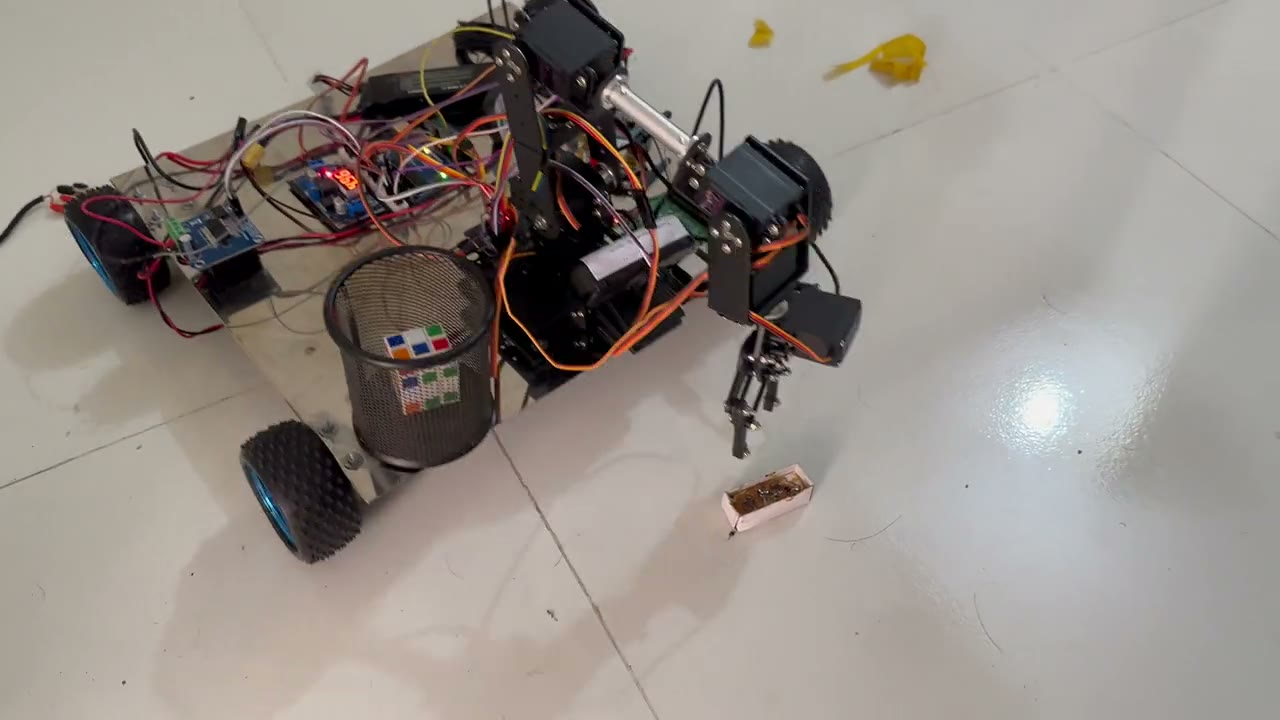
\includegraphics[height=44mm]{envirobot-2024-01-11-arm-and-motor-test-poster.jpg}\hfill
  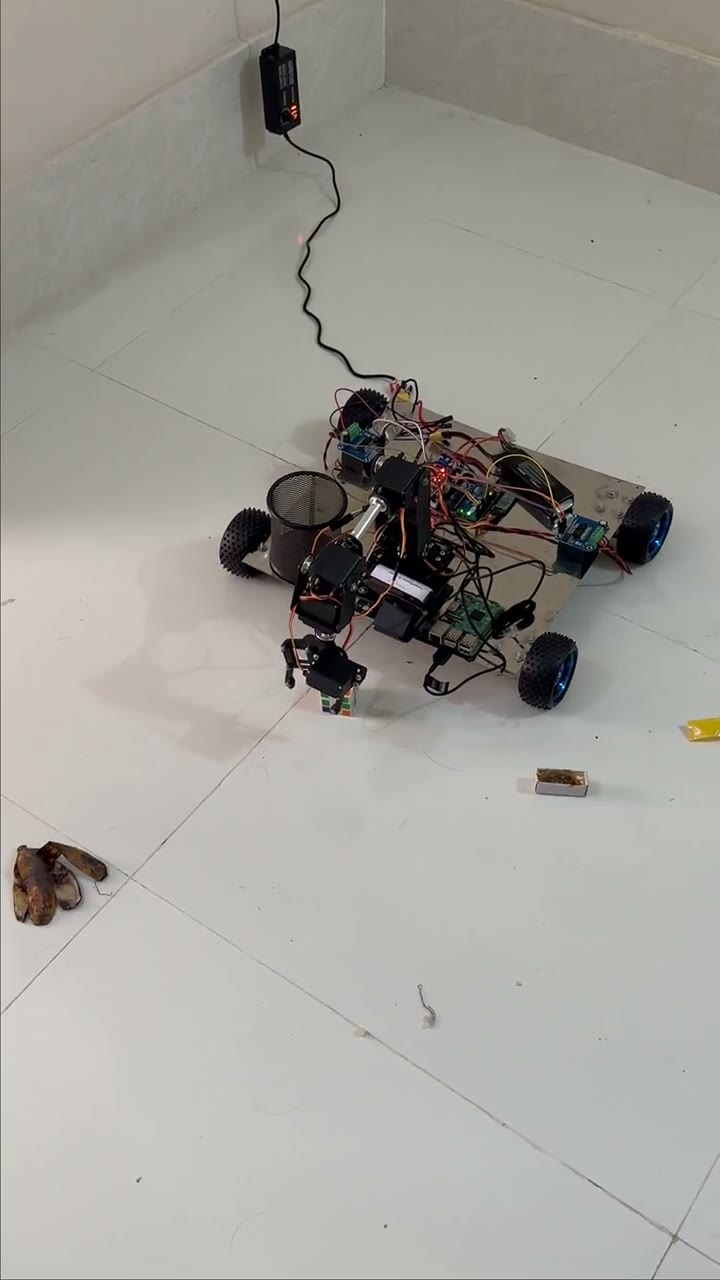
\includegraphics[height=44mm, trim=150 380 0 330, clip]{envirobot-2024-01-11-trash-collecting-frame.jpg}
  \caption{From the videos of 11 January 2024: the live detector boxing a spoon and naming it metal (left); the arm reaching for a box on the floor (middle); the gripper holding a cube it picked off the floor (right). In both arm videos the rover is on a power cable.}
  \label{fig:demo}
\end{figure}

The live test used a model that also names metal, which the three-class model in the report does not, so the live test ran a different version of the detector. The robot was presented at Comilla University in January 2024.

% ---------------------------------------------------------------------------
\section{Lessons Learned}

\paragraph{Build the base for the arm} The arm, not the rover, set the design: the team chose a steel base and four geared motors to carry it, at the cost of a heavier robot.

\paragraph{Split the work between two boards} Keeping all motion on the Arduino meant the arm and wheels could be driven from the phone on their own.

\paragraph{Manual control first} The phone app let the team test and calibrate every joint and the drive before any autonomy.

\paragraph{Reuse data, and name the metric} Starting from an earlier project's images and enlarging them with augmentation gave a usable detector. Recording which metric each number is, and keeping a set of background images, would have made the evaluation stronger.

% ---------------------------------------------------------------------------
\section{Limitations and Future Work}
\label{sec:future}

EnviroBot's detector was evaluated by the team in its report; its pick-ups and driving were recorded on video but not measured. The detector ran on a laptop in the recorded test, and the pick-up and the detector were shown separately. The repository holds the robot's model and ROS~2 package, while the detector, the Arduino code and the app stayed with the team.

Open steps follow from these (Fig.~\ref{fig:roadmap}): one program from the camera to the grasp, running the detector on the robot's own computer, and a measured pick-up success rate on a fixed set of objects; then driving a path and collecting on its own, and sorting waste into separate bins by class. The team's report also proposed Lidar for mapping and navigation, a depth camera to locate waste more precisely, and an industrial-grade arm.

\begin{figure}[htbp]
  \centering
  \diagramw{0.98}{figures/fig10-roadmap}
  \caption{What EnviroBot showed in 2024, and the open steps.}
  \label{fig:roadmap}
\end{figure}

% ---------------------------------------------------------------------------
\Needspace{8\baselineskip}
\section{Conclusion}

EnviroBot shows that a small team can build a mobile robot that finds waste and picks it up from low-cost parts: a steel rover, a six-servo arm, a Raspberry~Pi and an Arduino. Its YOLOv8 detector labelled plastic, paper and trash correctly more than nine times in ten in the team's evaluation, its arm picks objects off the floor, and the whole robot can be driven from a phone. Its model and ROS~2 package are open for others to build on.

% ---------------------------------------------------------------------------
\section*{Author Contributions}

All three authors designed, built and tested EnviroBot together at Comilla University. Jewel Nath put the robot's model into its public repository and wrote this report.

\section*{Acknowledgements}

The authors thank their supervisor, Amena Begum, Assistant Professor in the Department of Information and Communication Technology at Comilla University, for her guidance throughout the project.

The detector is built on Ultralytics YOLOv8 (AGPL-3.0). The ROS~2 package's test files come from the ROS~2 package template and keep the Open Source Robotics Foundation's Apache~2.0 notices.

This report was written with the help of AI assistants, under the first author's direction; its statements were checked against the team's report, the circuit diagram, the repository and the dated photos and videos.

{\small
\bibliographystyle{IEEEtran}
\bibliography{references}
}

% ---------------------------------------------------------------------------
\clearpage
\appendix
\section{Additional Material}

\begin{table}[!ht]
  \centering
  \caption{The repository.}
  \label{tab:repo}
  \renewcommand{\arraystretch}{1.25}
  \small
  \begin{tabularx}{0.92\textwidth}{@{}>{\ttfamily}p{0.34\textwidth}X@{}}
    \toprule
    \thead{Folder} & \thead{Holds} \\
    \midrule
    src/smart\_arm/description/ & the rover base and the arm in URDF/xacro, with their meshes \\
    src/smart\_arm/launch/ & a launch file that shows the rover base in RViz with a slider for each wheel; the arm's include is commented out \\
    src/smart\_arm/config/ & a ros2\_control controller set-up for the arm's six joints, not yet wired in \\
    src/smart\_arm/worlds/ & an empty Gazebo world \\
    docs/media/ & the photos and videos \\
    docs/report/ & this report, its figures and how to build it \\
    docs/diagrams/ & every diagram as its own PDF and PNG \\
    \bottomrule
  \end{tabularx}
\end{table}

\end{document}
